\documentclass[]{article}
\usepackage{lmodern}
\usepackage{amssymb,amsmath}
\usepackage{ifxetex,ifluatex}
\usepackage{fixltx2e} % provides \textsubscript
\ifnum 0\ifxetex 1\fi\ifluatex 1\fi=0 % if pdftex
  \usepackage[T1]{fontenc}
  \usepackage[utf8]{inputenc}
\else % if luatex or xelatex
  \ifxetex
    \usepackage{mathspec}
  \else
    \usepackage{fontspec}
  \fi
  \defaultfontfeatures{Ligatures=TeX,Scale=MatchLowercase}
\fi
% use upquote if available, for straight quotes in verbatim environments
\IfFileExists{upquote.sty}{\usepackage{upquote}}{}
% use microtype if available
\IfFileExists{microtype.sty}{%
\usepackage{microtype}
\UseMicrotypeSet[protrusion]{basicmath} % disable protrusion for tt fonts
}{}
\usepackage[margin=1in]{geometry}
\usepackage{hyperref}
\hypersetup{unicode=true,
            pdftitle={FE8828 Programming Web Applications in Finance},
            pdfauthor={Dr.~Yang Ye  \textless Email:yy@runchee.com\textgreater{}},
            pdfborder={0 0 0},
            breaklinks=true}
\urlstyle{same}  % don't use monospace font for urls
\usepackage{color}
\usepackage{fancyvrb}
\newcommand{\VerbBar}{|}
\newcommand{\VERB}{\Verb[commandchars=\\\{\}]}
\DefineVerbatimEnvironment{Highlighting}{Verbatim}{commandchars=\\\{\}}
% Add ',fontsize=\small' for more characters per line
\usepackage{framed}
\definecolor{shadecolor}{RGB}{248,248,248}
\newenvironment{Shaded}{\begin{snugshade}}{\end{snugshade}}
\newcommand{\AlertTok}[1]{\textcolor[rgb]{0.94,0.16,0.16}{#1}}
\newcommand{\AnnotationTok}[1]{\textcolor[rgb]{0.56,0.35,0.01}{\textbf{\textit{#1}}}}
\newcommand{\AttributeTok}[1]{\textcolor[rgb]{0.77,0.63,0.00}{#1}}
\newcommand{\BaseNTok}[1]{\textcolor[rgb]{0.00,0.00,0.81}{#1}}
\newcommand{\BuiltInTok}[1]{#1}
\newcommand{\CharTok}[1]{\textcolor[rgb]{0.31,0.60,0.02}{#1}}
\newcommand{\CommentTok}[1]{\textcolor[rgb]{0.56,0.35,0.01}{\textit{#1}}}
\newcommand{\CommentVarTok}[1]{\textcolor[rgb]{0.56,0.35,0.01}{\textbf{\textit{#1}}}}
\newcommand{\ConstantTok}[1]{\textcolor[rgb]{0.00,0.00,0.00}{#1}}
\newcommand{\ControlFlowTok}[1]{\textcolor[rgb]{0.13,0.29,0.53}{\textbf{#1}}}
\newcommand{\DataTypeTok}[1]{\textcolor[rgb]{0.13,0.29,0.53}{#1}}
\newcommand{\DecValTok}[1]{\textcolor[rgb]{0.00,0.00,0.81}{#1}}
\newcommand{\DocumentationTok}[1]{\textcolor[rgb]{0.56,0.35,0.01}{\textbf{\textit{#1}}}}
\newcommand{\ErrorTok}[1]{\textcolor[rgb]{0.64,0.00,0.00}{\textbf{#1}}}
\newcommand{\ExtensionTok}[1]{#1}
\newcommand{\FloatTok}[1]{\textcolor[rgb]{0.00,0.00,0.81}{#1}}
\newcommand{\FunctionTok}[1]{\textcolor[rgb]{0.00,0.00,0.00}{#1}}
\newcommand{\ImportTok}[1]{#1}
\newcommand{\InformationTok}[1]{\textcolor[rgb]{0.56,0.35,0.01}{\textbf{\textit{#1}}}}
\newcommand{\KeywordTok}[1]{\textcolor[rgb]{0.13,0.29,0.53}{\textbf{#1}}}
\newcommand{\NormalTok}[1]{#1}
\newcommand{\OperatorTok}[1]{\textcolor[rgb]{0.81,0.36,0.00}{\textbf{#1}}}
\newcommand{\OtherTok}[1]{\textcolor[rgb]{0.56,0.35,0.01}{#1}}
\newcommand{\PreprocessorTok}[1]{\textcolor[rgb]{0.56,0.35,0.01}{\textit{#1}}}
\newcommand{\RegionMarkerTok}[1]{#1}
\newcommand{\SpecialCharTok}[1]{\textcolor[rgb]{0.00,0.00,0.00}{#1}}
\newcommand{\SpecialStringTok}[1]{\textcolor[rgb]{0.31,0.60,0.02}{#1}}
\newcommand{\StringTok}[1]{\textcolor[rgb]{0.31,0.60,0.02}{#1}}
\newcommand{\VariableTok}[1]{\textcolor[rgb]{0.00,0.00,0.00}{#1}}
\newcommand{\VerbatimStringTok}[1]{\textcolor[rgb]{0.31,0.60,0.02}{#1}}
\newcommand{\WarningTok}[1]{\textcolor[rgb]{0.56,0.35,0.01}{\textbf{\textit{#1}}}}
\usepackage{graphicx,grffile}
\makeatletter
\def\maxwidth{\ifdim\Gin@nat@width>\linewidth\linewidth\else\Gin@nat@width\fi}
\def\maxheight{\ifdim\Gin@nat@height>\textheight\textheight\else\Gin@nat@height\fi}
\makeatother
% Scale images if necessary, so that they will not overflow the page
% margins by default, and it is still possible to overwrite the defaults
% using explicit options in \includegraphics[width, height, ...]{}
\setkeys{Gin}{width=\maxwidth,height=\maxheight,keepaspectratio}
\IfFileExists{parskip.sty}{%
\usepackage{parskip}
}{% else
\setlength{\parindent}{0pt}
\setlength{\parskip}{6pt plus 2pt minus 1pt}
}
\setlength{\emergencystretch}{3em}  % prevent overfull lines
\providecommand{\tightlist}{%
  \setlength{\itemsep}{0pt}\setlength{\parskip}{0pt}}
\setcounter{secnumdepth}{0}
% Redefines (sub)paragraphs to behave more like sections
\ifx\paragraph\undefined\else
\let\oldparagraph\paragraph
\renewcommand{\paragraph}[1]{\oldparagraph{#1}\mbox{}}
\fi
\ifx\subparagraph\undefined\else
\let\oldsubparagraph\subparagraph
\renewcommand{\subparagraph}[1]{\oldsubparagraph{#1}\mbox{}}
\fi

%%% Use protect on footnotes to avoid problems with footnotes in titles
\let\rmarkdownfootnote\footnote%
\def\footnote{\protect\rmarkdownfootnote}

%%% Change title format to be more compact
\usepackage{titling}

% Create subtitle command for use in maketitle
\providecommand{\subtitle}[1]{
  \posttitle{
    \begin{center}\large#1\end{center}
    }
}

\setlength{\droptitle}{-2em}

  \title{FE8828 Programming Web Applications in Finance}
    \pretitle{\vspace{\droptitle}\centering\huge}
  \posttitle{\par}
  \subtitle{Session 5 Building Financial Applications}
  \author{Dr.~Yang Ye
\textless Email:\href{mailto:yy@runchee.com}{\nolinkurl{yy@runchee.com}}\textgreater{}}
    \preauthor{\centering\large\emph}
  \postauthor{\par}
      \predate{\centering\large\emph}
  \postdate{\par}
    \date{Sep 24, 2019}


\begin{document}
\maketitle

\hypertarget{lecture-10-building-financial-applications}{%
\section{Lecture 10: Building Financial
Applications}\label{lecture-10-building-financial-applications}}

\hypertarget{starter}{%
\section{Starter}\label{starter}}

\begin{Shaded}
\begin{Highlighting}[]
\CommentTok{# biorhythm.R}

\KeywordTok{library}\NormalTok{(dplyr)}
\KeywordTok{library}\NormalTok{(tidyr)}
\KeywordTok{library}\NormalTok{(ggplot2)}

\NormalTok{biorhythm <-}\StringTok{ }\ControlFlowTok{function}\NormalTok{(dob, }\DataTypeTok{target =} \KeywordTok{Sys.Date}\NormalTok{()) \{}
\NormalTok{  dob <-}\StringTok{ }\KeywordTok{as.Date}\NormalTok{(dob)}
\NormalTok{  target <-}\StringTok{ }\KeywordTok{as.Date}\NormalTok{(target)}
\NormalTok{  t <-}\StringTok{ }\KeywordTok{round}\NormalTok{(}\KeywordTok{as.numeric}\NormalTok{(}\KeywordTok{difftime}\NormalTok{(target, dob)))}
\NormalTok{  days <-}\StringTok{ }\NormalTok{(t }\OperatorTok{-}\StringTok{ }\DecValTok{14}\NormalTok{) }\OperatorTok{:}\StringTok{ }\NormalTok{(t }\OperatorTok{+}\StringTok{ }\DecValTok{14}\NormalTok{)}
\NormalTok{  period <-}\StringTok{ }\KeywordTok{tibble}\NormalTok{(}\DataTypeTok{Date =} \KeywordTok{seq.Date}\NormalTok{(}\DataTypeTok{from =}\NormalTok{ target }\OperatorTok{-}\StringTok{ }\DecValTok{15}\NormalTok{, }\DataTypeTok{by =} \DecValTok{1}\NormalTok{, }\DataTypeTok{length.out =} \DecValTok{29}\NormalTok{),}
                       \DataTypeTok{Physical =} \KeywordTok{sin}\NormalTok{ (}\DecValTok{2} \OperatorTok{*}\StringTok{ }\NormalTok{pi }\OperatorTok{*}\StringTok{ }\NormalTok{days }\OperatorTok{/}\StringTok{ }\DecValTok{23}\NormalTok{) }\OperatorTok{*}\StringTok{ }\DecValTok{100}\NormalTok{, }
                       \DataTypeTok{Emotional =} \KeywordTok{sin}\NormalTok{ (}\DecValTok{2} \OperatorTok{*}\StringTok{ }\NormalTok{pi }\OperatorTok{*}\StringTok{ }\NormalTok{days }\OperatorTok{/}\StringTok{ }\DecValTok{28}\NormalTok{) }\OperatorTok{*}\StringTok{ }\DecValTok{100}\NormalTok{, }
                       \DataTypeTok{Intellectual =} \KeywordTok{sin}\NormalTok{ (}\DecValTok{2} \OperatorTok{*}\StringTok{ }\NormalTok{pi }\OperatorTok{*}\StringTok{ }\NormalTok{days }\OperatorTok{/}\StringTok{ }\DecValTok{33}\NormalTok{) }\OperatorTok{*}\StringTok{ }\DecValTok{100}\NormalTok{)}
\NormalTok{  period <-}\StringTok{ }\KeywordTok{gather}\NormalTok{(period, }\DataTypeTok{key =} \StringTok{"Biorhythm"}\NormalTok{, }\DataTypeTok{value =} \StringTok{"Percentage"}\NormalTok{, }\OperatorTok{-}\NormalTok{Date)}
  \KeywordTok{ggplot}\NormalTok{(period, }\KeywordTok{aes}\NormalTok{(}\DataTypeTok{x =}\NormalTok{ Date, }\DataTypeTok{y =}\NormalTok{ Percentage, }\DataTypeTok{col =}\NormalTok{ Biorhythm)) }\OperatorTok{+}
\StringTok{    }\KeywordTok{geom_line}\NormalTok{() }\OperatorTok{+}\StringTok{  }
\StringTok{    }\KeywordTok{ggtitle}\NormalTok{(}\KeywordTok{paste}\NormalTok{(}\StringTok{"DoB:"}\NormalTok{, }\KeywordTok{format}\NormalTok{(dob, }\StringTok{"%d %B %Y"}\NormalTok{))) }\OperatorTok{+}\StringTok{ }
\StringTok{    }\KeywordTok{geom_vline}\NormalTok{(}\DataTypeTok{xintercept =} \KeywordTok{as.numeric}\NormalTok{(target)) }\OperatorTok{+}
\StringTok{    }\KeywordTok{theme}\NormalTok{(}\DataTypeTok{legend.position =} \StringTok{"bottom"}\NormalTok{)}
\NormalTok{\}}
\end{Highlighting}
\end{Shaded}

\hypertarget{starter---result}{%
\section{Starter - Result}\label{starter---result}}

\begin{Shaded}
\begin{Highlighting}[]
\CommentTok{# I took four people's birthdays. Hope they are in good mood today.}
\NormalTok{g1 <-}\StringTok{ }\KeywordTok{biorhythm}\NormalTok{(}\StringTok{"1964-01-12"}\NormalTok{, }\KeywordTok{Sys.Date}\NormalTok{())}
\NormalTok{g2 <-}\StringTok{ }\KeywordTok{biorhythm}\NormalTok{(}\StringTok{"1971-06-28"}\NormalTok{, }\KeywordTok{Sys.Date}\NormalTok{())}
\NormalTok{g3 <-}\StringTok{ }\KeywordTok{biorhythm}\NormalTok{(}\StringTok{"1971-10-29"}\NormalTok{, }\KeywordTok{Sys.Date}\NormalTok{())}
\NormalTok{g4 <-}\StringTok{ }\KeywordTok{biorhythm}\NormalTok{(}\StringTok{"1957-08-11"}\NormalTok{, }\KeywordTok{Sys.Date}\NormalTok{())}
\KeywordTok{grid.arrange}\NormalTok{(g1, g2, g3, g4, }\DataTypeTok{ncol =} \DecValTok{2}\NormalTok{, }\DataTypeTok{nrow =} \DecValTok{2}\NormalTok{)}
\end{Highlighting}
\end{Shaded}

\begin{center}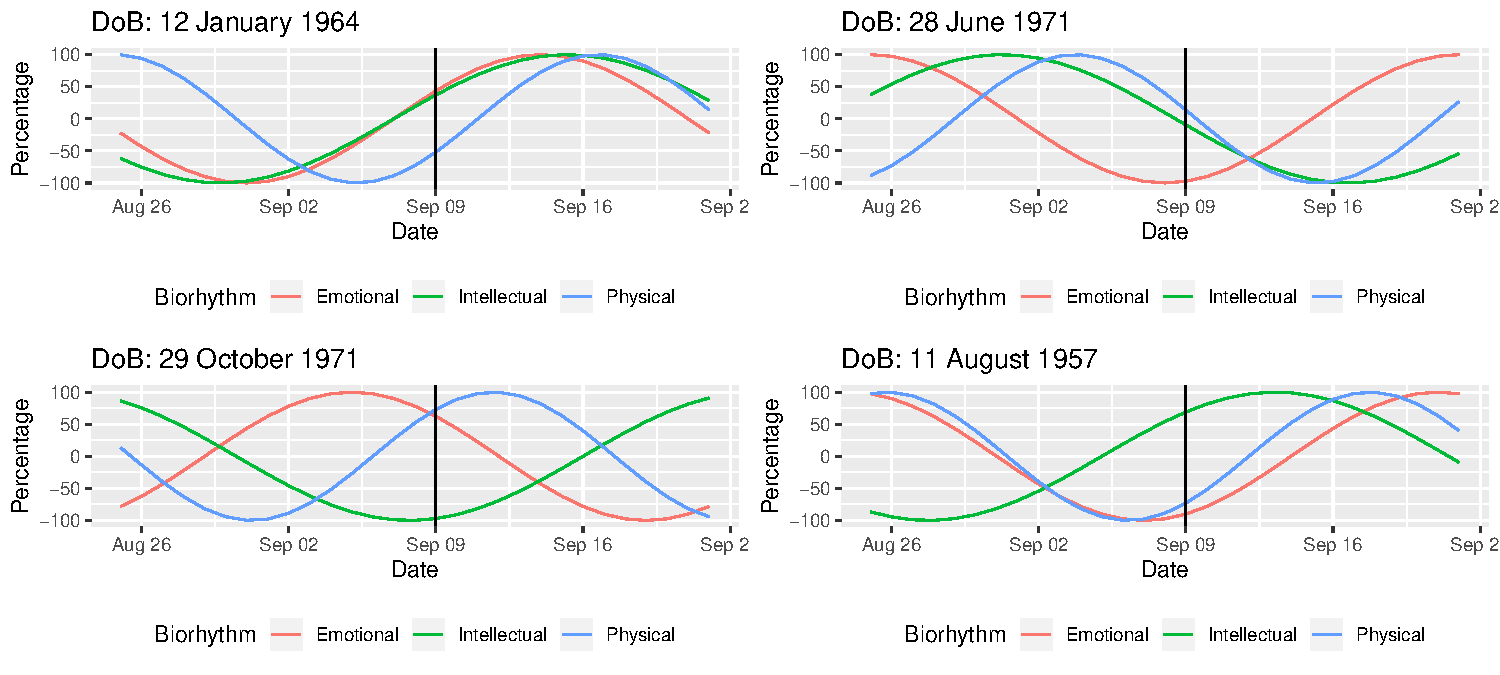
\includegraphics{lec13_files/figure-latex/unnamed-chunk-3-1} \end{center}

\hypertarget{main-course}{%
\section{Main course}\label{main-course}}

\begin{itemize}
\tightlist
\item
  We need following packages as a start. Use c() to install multiple
  packages.
\end{itemize}

\begin{Shaded}
\begin{Highlighting}[]
\KeywordTok{install.packages}\NormalTok{(}\KeywordTok{c}\NormalTok{(}\StringTok{"tidyquant"}\NormalTok{, }\StringTok{"Quandl"}\NormalTok{, }\StringTok{"fOptions"}\NormalTok{, }\StringTok{"fExoticOptions"}\NormalTok{, }\StringTok{"dygraph"}\NormalTok{, }\StringTok{"forecast"}\NormalTok{))}
\end{Highlighting}
\end{Shaded}

\begin{itemize}
\item
  \texttt{tidyquant} is also a collection of packages: \texttt{xts},
  \texttt{quantmod}.
\item
  Please validate option pricing code.

  \begin{itemize}
  \tightlist
  \item
    For example, I found Asian Option
    \texttt{TurnbullWakemanAsianApproxOption()} in
    \texttt{fExoticOptions} is strangely implemented. Maybe I am wrong.
  \end{itemize}
\end{itemize}

\hypertarget{tidyquant-or-quandl}{%
\section{tidyquant or Quandl?}\label{tidyquant-or-quandl}}

Determining factors:

\begin{itemize}
\tightlist
\item
  \texttt{tidyquant/quantmod} can connect to various services:
  \textsubscript{google}, yahoo (still active), av (AlphaAdvantage).
\item
  Quandl only connects to Quandl
\item
  It's subjected to where you can find the data.

  \begin{itemize}
  \tightlist
  \item
    US ETF/Stocks on Quandl is a premium service.
  \item
    ETF in Google/AlphaAdvantage is free.
  \end{itemize}
\end{itemize}

\hypertarget{tidyquant-or-quandl-1}{%
\section{tidyquant or Quandl?}\label{tidyquant-or-quandl-1}}

Technical details:

\begin{itemize}
\tightlist
\item
  quantmod returns \texttt{xts} object. Quandl returns data frame or
  \texttt{xts}
\item
  xts object is can \texttt{collapse} to daily, weekly, monthly price.
\end{itemize}

\hypertarget{tidyquantquantmod}{%
\section{Tidyquant/quantmod}\label{tidyquantquantmod}}

\begin{Shaded}
\begin{Highlighting}[]
\CommentTok{# library(tidyquant)}

\CommentTok{# use Google}
\KeywordTok{getSymbols}\NormalTok{(}\StringTok{'SPY'}\NormalTok{, }\DataTypeTok{src =} \StringTok{'yahoo'}\NormalTok{, }\DataTypeTok{adjusted =} \OtherTok{TRUE}\NormalTok{, }\DataTypeTok{output.size =} \StringTok{'full'}\NormalTok{)}
\CommentTok{## Warning: SPY download failed; trying again.}
\CommentTok{## [1] "SPY"}
\KeywordTok{str}\NormalTok{(SPY)}
\CommentTok{## An 'xts' object on 2007-01-03/2019-09-06 containing:}
\CommentTok{##   Data: num [1:3192, 1:6] 142 141 141 141 141 ...}
\CommentTok{##  - attr(*, "dimnames")=List of 2}
\CommentTok{##   ..$ : NULL}
\CommentTok{##   ..$ : chr [1:6] "SPY.Open" "SPY.High" "SPY.Low" "SPY.Close" ...}
\CommentTok{##   Indexed by objects of class: [Date] TZ: UTC}
\CommentTok{##   xts Attributes:  }
\CommentTok{## List of 2}
\CommentTok{##  $ src    : chr "yahoo"}
\CommentTok{##  $ updated: POSIXct[1:1], format: "2019-09-09 21:14:22"}

\CommentTok{# Sign up with AlphaAdvantage to get a token}
\CommentTok{# getSymbols('SPY', src = 'av', output.size = 'full', api.key = token_av)}
\CommentTok{# str(SPY)}
\end{Highlighting}
\end{Shaded}

\hypertarget{tidyquantquantmod-1}{%
\section{Tidyquant/quantmod}\label{tidyquantquantmod-1}}

\begin{Shaded}
\begin{Highlighting}[]
\CommentTok{# What's get returned?}
\KeywordTok{head}\NormalTok{(SPY)}
\CommentTok{##            SPY.Open SPY.High SPY.Low SPY.Close SPY.Volume SPY.Adjusted}
\CommentTok{## 2007-01-03   142.25   142.86  140.57    141.37   94807600     109.5033}
\CommentTok{## 2007-01-04   141.23   142.05  140.61    141.67   69620600     109.7357}
\CommentTok{## 2007-01-05   141.33   141.40  140.38    140.54   76645300     108.8604}
\CommentTok{## 2007-01-08   140.82   141.41  140.25    141.19   71655000     109.3639}
\CommentTok{## 2007-01-09   141.31   141.60  140.40    141.07   75680100     109.2709}
\CommentTok{## 2007-01-10   140.58   141.57  140.30    141.54   72428000     109.6350}
\KeywordTok{tail}\NormalTok{(SPY)}
\CommentTok{##            SPY.Open SPY.High SPY.Low SPY.Close SPY.Volume SPY.Adjusted}
\CommentTok{## 2019-08-29   291.72   293.16  290.61    292.58   57899400       292.58}
\CommentTok{## 2019-08-30   294.22   294.24  291.42    292.45   62901200       292.45}
\CommentTok{## 2019-09-03   290.57   291.58  289.27    290.74   69101400       290.74}
\CommentTok{## 2019-09-04   293.14   294.06  292.31    294.04   46887300       294.04}
\CommentTok{## 2019-09-05   296.79   298.83  294.00    297.82   83258100       297.82}
\CommentTok{## 2019-09-06   298.17   298.76  297.42    298.05   49522600       298.05}

\NormalTok{symbols <-}\StringTok{ }\KeywordTok{c}\NormalTok{(}\StringTok{"MSFT"}\NormalTok{, }\StringTok{"AAPL"}\NormalTok{)}
\KeywordTok{getSymbols}\NormalTok{(symbols, }\DataTypeTok{src =} \StringTok{'yahoo'}\NormalTok{, }\DataTypeTok{adjusted =} \OtherTok{TRUE}\NormalTok{, }\DataTypeTok{from =} \StringTok{"2016-01-01"}\NormalTok{)}
\CommentTok{## [1] "MSFT" "AAPL"}
\end{Highlighting}
\end{Shaded}

\hypertarget{xts-object}{%
\section{\texorpdfstring{\texttt{xts}
object}{xts object}}\label{xts-object}}

\begin{itemize}
\tightlist
\item
  xts is a wide format. In contrast, ggplot/tidy uses long format.
\item
  We have gather/spread to convert between long/wide format.
\item
  Create xts object:

  \begin{itemize}
  \tightlist
  \item
    Put index aside, which is usually date
  \item
    Store prices in columns.
  \end{itemize}
\end{itemize}

\begin{Shaded}
\begin{Highlighting}[]
\KeywordTok{library}\NormalTok{(xts)}

\CommentTok{# if df is a data frame.}
\CommentTok{# Date | V | GS}
\NormalTok{xts1 <-}\StringTok{ }\KeywordTok{xts}\NormalTok{(}\DataTypeTok{x=}\NormalTok{df[, }\DecValTok{-1}\NormalTok{, }\DataTypeTok{drop =}\NormalTok{ F], }\DataTypeTok{order.by =}\NormalTok{ df[}\DecValTok{1}\NormalTok{])}

\CommentTok{# coredata: returns a matrix from xts objects}
\NormalTok{core_data <-}\StringTok{ }\KeywordTok{coredata}\NormalTok{(xts2)}

\CommentTok{# index: vector of any Date, POSIXct, chron, yearmon, yearqtr, or DateTime classes}
\KeywordTok{index}\NormalTok{(xts1)}
\end{Highlighting}
\end{Shaded}

\hypertarget{get-data-from-xts-object}{%
\section{\texorpdfstring{Get data from \texttt{xts}
object}{Get data from xts object}}\label{get-data-from-xts-object}}

\begin{Shaded}
\begin{Highlighting}[]
\CommentTok{# What price history is stored here.}
\KeywordTok{str}\NormalTok{(SPY)}
\CommentTok{## An 'xts' object on 2007-01-03/2019-09-06 containing:}
\CommentTok{##   Data: num [1:3192, 1:6] 142 141 141 141 141 ...}
\CommentTok{##  - attr(*, "dimnames")=List of 2}
\CommentTok{##   ..$ : NULL}
\CommentTok{##   ..$ : chr [1:6] "SPY.Open" "SPY.High" "SPY.Low" "SPY.Close" ...}
\CommentTok{##   Indexed by objects of class: [Date] TZ: UTC}
\CommentTok{##   xts Attributes:  }
\CommentTok{## List of 2}
\CommentTok{##  $ src    : chr "yahoo"}
\CommentTok{##  $ updated: POSIXct[1:1], format: "2019-09-09 21:14:22"}
\end{Highlighting}
\end{Shaded}

\begin{Shaded}
\begin{Highlighting}[]
\NormalTok{SPY2003 <-}\StringTok{ }\NormalTok{SPY[}\StringTok{"2003"}\NormalTok{]}
\NormalTok{SPY2 <-}\StringTok{ }\NormalTok{SPY[}\StringTok{"2003/2007"}\NormalTok{]}
\NormalTok{SPY3 <-}\StringTok{ }\NormalTok{SPY[}\StringTok{"2003-03-01/2007-07-01"}\NormalTok{]}
\NormalTok{SPY4 <-}\StringTok{ }\NormalTok{SPY[}\StringTok{"/2007-07-01"}\NormalTok{] }\CommentTok{# till }
\NormalTok{SPY5 <-}\StringTok{ }\NormalTok{SPY[}\StringTok{"2007-07-01/"}\NormalTok{] }\CommentTok{# from}
\NormalTok{SPY6 <-}\StringTok{ }\NormalTok{SPY[}\StringTok{"2007-07-01/"}\NormalTok{, }\StringTok{"SPY.High"}\NormalTok{]}
\NormalTok{SPY7 <-}\StringTok{ }\NormalTok{SPY[}\StringTok{"2007-07-01/"}\NormalTok{, }\KeywordTok{c}\NormalTok{(}\StringTok{"SPY.High"}\NormalTok{, }\StringTok{"SPY.Close"}\NormalTok{)]}
\end{Highlighting}
\end{Shaded}

\hypertarget{quandl}{%
\section{Quandl}\label{quandl}}

\begin{Shaded}
\begin{Highlighting}[]
\KeywordTok{library}\NormalTok{(Quandl)}
\KeywordTok{library}\NormalTok{(tidyverse)}

\CommentTok{# Sign up with Quandl to get a token}
\CommentTok{# token_qd <- "xxxx"}
\KeywordTok{Quandl.api_key}\NormalTok{(token_qd)}
\CommentTok{## You don't get SPY: SPDR 500 ETF from Quandl from free service.}
\CommentTok{## rates <- Quandl(c("EOD/SPY"), start_date="2000-01-01", end_date="2013-06-07")}
\CommentTok{## You don't get EOD US Stocks for free from Quandl from 2019}
\CommentTok{## rates <- Quandl(c("EOD/V"), start_date="2000-01-01", end_date="2013-06-07" )}
\end{Highlighting}
\end{Shaded}

\hypertarget{quandl-1}{%
\section{Quandl}\label{quandl-1}}

\begin{Shaded}
\begin{Highlighting}[]
\KeywordTok{library}\NormalTok{(Quandl)                 }\CommentTok{# Quandl package}
\KeywordTok{library}\NormalTok{(ggplot2)                }\CommentTok{# Package for plotting}
\KeywordTok{library}\NormalTok{(tidyverse)              }\CommentTok{# Package for reshaping data}

\KeywordTok{Quandl.api_key}\NormalTok{(token_qd)                }\CommentTok{# Authenticate your token}
\CommentTok{# Build vector of currencies}
\NormalTok{rates <-}\StringTok{ }\KeywordTok{Quandl}\NormalTok{(}\KeywordTok{c}\NormalTok{(}\StringTok{"FRED/DEXUSAL"}\NormalTok{, }\StringTok{"FRED/DEXBZUS"}\NormalTok{, }\StringTok{"FRED/DEXUSUK"}\NormalTok{, }\StringTok{"FRED/DEXCHUS"}\NormalTok{),}
                \DataTypeTok{start_date=}\StringTok{"2000-01-01"}\NormalTok{,}
                \DataTypeTok{end_date =} \StringTok{"2018-11-28"}\NormalTok{)}
\KeywordTok{colnames}\NormalTok{(rates) <-}\StringTok{ }\KeywordTok{c}\NormalTok{(}\StringTok{"Date"}\NormalTok{, }\StringTok{"AUD/USD"}\NormalTok{, }\StringTok{"USD/BRL"}\NormalTok{, }\StringTok{"GBP/USD"}\NormalTok{, }\StringTok{"USD/CNY"}\NormalTok{)}
\NormalTok{meltdf <-}\StringTok{ }\KeywordTok{gather}\NormalTok{(rates, }\DataTypeTok{key =} \StringTok{"CCY"}\NormalTok{, }\DataTypeTok{value =} \StringTok{"Rate"}\NormalTok{, }\OperatorTok{-}\NormalTok{Date)}

\KeywordTok{ggplot}\NormalTok{(meltdf, }\KeywordTok{aes}\NormalTok{(}\DataTypeTok{x =}\NormalTok{ Date, }\DataTypeTok{y =}\NormalTok{ Rate, }\DataTypeTok{colour =}\NormalTok{ CCY, }\DataTypeTok{group =}\NormalTok{ CCY)) }\OperatorTok{+}
\StringTok{  }\KeywordTok{geom_line}\NormalTok{() }\OperatorTok{+}
\StringTok{  }\KeywordTok{scale_colour_manual}\NormalTok{(}\DataTypeTok{values=}\DecValTok{1}\OperatorTok{:}\DecValTok{22}\NormalTok{)}\OperatorTok{+}
\StringTok{  }\KeywordTok{ggtitle}\NormalTok{(}\StringTok{"Major Currency Exchange Rates in USD"}\NormalTok{) }\OperatorTok{+}
\StringTok{  }\KeywordTok{theme_minimal}\NormalTok{()}
\end{Highlighting}
\end{Shaded}

\begin{center}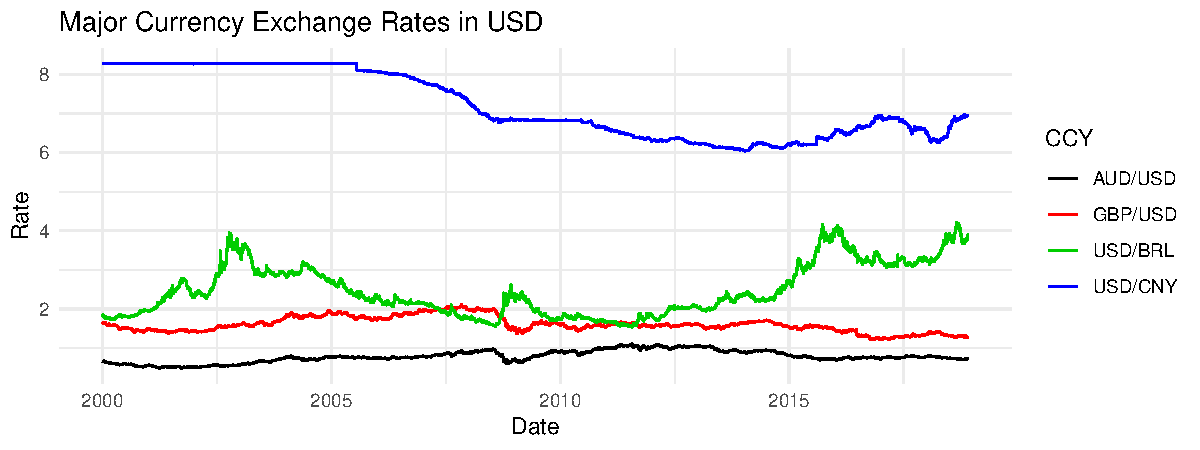
\includegraphics{lec13_files/figure-latex/unnamed-chunk-11-1} \end{center}

\hypertarget{quandl-and-forecast}{%
\section{Quandl and forecast}\label{quandl-and-forecast}}

\begin{Shaded}
\begin{Highlighting}[]
\CommentTok{# 52-quandl-forecast.R}
\CommentTok{# Quandl and Forecast}
\CommentTok{# Forecast using state space models and automatic ARIMA modelling.}

\KeywordTok{library}\NormalTok{(Quandl)}
\KeywordTok{library}\NormalTok{(dplyr)}
\KeywordTok{library}\NormalTok{(xts)}
\KeywordTok{library}\NormalTok{(lubridate)}
\KeywordTok{library}\NormalTok{(forecast)}
\KeywordTok{library}\NormalTok{(dygraphs)}

\CommentTok{# Start with daily data. Note that "type = raw" will download a data frame.}
\NormalTok{oil_daily <-}\StringTok{ }\KeywordTok{Quandl}\NormalTok{(}\StringTok{"FRED/DCOILWTICO"}\NormalTok{, }\DataTypeTok{type =} \StringTok{"raw"}\NormalTok{, }\DataTypeTok{collapse =} \StringTok{"daily"}\NormalTok{,  }
                    \DataTypeTok{start_date=}\StringTok{"2006-01-01"}\NormalTok{, }\DataTypeTok{end_date=}\KeywordTok{Sys.Date}\NormalTok{())}
\CommentTok{# Now weekely and let's use xts as the type.}
\NormalTok{oil_weekly <-}\StringTok{ }\KeywordTok{Quandl}\NormalTok{(}\StringTok{"FRED/DCOILWTICO"}\NormalTok{, }\DataTypeTok{type =} \StringTok{"xts"}\NormalTok{, }\DataTypeTok{collapse =} \StringTok{"weekly"}\NormalTok{,}
                     \DataTypeTok{start_date=}\StringTok{"2006-01-01"}\NormalTok{, }\DataTypeTok{end_date =} \KeywordTok{Sys.Date}\NormalTok{())}
\NormalTok{oil_monthly <-}\StringTok{ }\KeywordTok{Quandl}\NormalTok{(}\StringTok{"FRED/DCOILWTICO"}\NormalTok{, }\DataTypeTok{type =} \StringTok{"xts"}\NormalTok{, }\DataTypeTok{collapse =} \StringTok{"monthly"}\NormalTok{,}
                      \DataTypeTok{start_date=}\StringTok{"2006-01-01"}\NormalTok{, }\DataTypeTok{end_date =} \KeywordTok{Sys.Date}\NormalTok{())}

\CommentTok{# Have a quick look at our three  objects. }
\KeywordTok{str}\NormalTok{(oil_daily)}
\KeywordTok{str}\NormalTok{(oil_weekly)}
\KeywordTok{str}\NormalTok{(oil_monthly)}

\KeywordTok{cat}\NormalTok{(}\KeywordTok{paste0}\NormalTok{(}\StringTok{"daily: "}\NormalTok{, }\KeywordTok{paste0}\NormalTok{(}\KeywordTok{range}\NormalTok{(oil_daily}\OperatorTok{$}\NormalTok{Date), }\DataTypeTok{collapse =} \StringTok{", "}\NormalTok{), }\StringTok{"}\CharTok{\textbackslash{}n}\StringTok{"}\NormalTok{))}
\KeywordTok{cat}\NormalTok{(}\KeywordTok{paste0}\NormalTok{(}\StringTok{"weekly: "}\NormalTok{, }\KeywordTok{paste0}\NormalTok{(}\KeywordTok{range}\NormalTok{(}\KeywordTok{index}\NormalTok{(oil_weekly)), }\DataTypeTok{collapse =} \StringTok{", "}\NormalTok{), }\StringTok{"}\CharTok{\textbackslash{}n}\StringTok{"}\NormalTok{))}
\KeywordTok{cat}\NormalTok{(}\KeywordTok{paste0}\NormalTok{(}\StringTok{"monthly: "}\NormalTok{, }\KeywordTok{paste0}\NormalTok{(}\KeywordTok{range}\NormalTok{(}\KeywordTok{index}\NormalTok{(oil_monthly)), }\DataTypeTok{collapse =} \StringTok{", "}\NormalTok{), }\StringTok{"}\CharTok{\textbackslash{}n}\StringTok{"}\NormalTok{))}

\CommentTok{# Change index from month to day}
\KeywordTok{head}\NormalTok{(}\KeywordTok{index}\NormalTok{(oil_monthly))}
\KeywordTok{index}\NormalTok{(oil_monthly) <-}\StringTok{ }\KeywordTok{seq}\NormalTok{(}\KeywordTok{mdy}\NormalTok{(}\StringTok{'01/01/2006'}\NormalTok{), }\KeywordTok{Sys.Date}\NormalTok{(), }\DataTypeTok{by =} \StringTok{'months'}\NormalTok{)[}\DecValTok{1}\OperatorTok{:}\KeywordTok{length}\NormalTok{(oil_monthly)]}
\CommentTok{# index(oil_monthly) <- seq(mdy('01/01/2006'), (Sys.Date() - 365 * 2), by = 'months')}
\KeywordTok{str}\NormalTok{(oil_monthly)}
\KeywordTok{head}\NormalTok{(}\KeywordTok{index}\NormalTok{(oil_monthly))}

\KeywordTok{dygraph}\NormalTok{(oil_monthly, }\DataTypeTok{main =} \StringTok{"Monthly oil Prices"}\NormalTok{)}

\NormalTok{forebase1 <-}\StringTok{ }\NormalTok{oil_weekly[}\KeywordTok{paste0}\NormalTok{(}\StringTok{"/"}\NormalTok{, }\KeywordTok{Sys.Date}\NormalTok{() }\OperatorTok{-}\StringTok{ }\DecValTok{365} \OperatorTok{*}\StringTok{ }\DecValTok{2}\NormalTok{)]}
\NormalTok{forecast1 <-}\StringTok{ }\KeywordTok{forecast}\NormalTok{(forebase1, }\DataTypeTok{h =} \DecValTok{4} \OperatorTok{*}\StringTok{ }\DecValTok{24}\NormalTok{)}

\KeywordTok{plot}\NormalTok{(forecast1, }\DataTypeTok{main =} \StringTok{"Oil Forecast1"}\NormalTok{)}

\NormalTok{oil_forecast_data1 <-}\StringTok{ }\KeywordTok{data.frame}\NormalTok{(}\DataTypeTok{date =} \KeywordTok{seq}\NormalTok{(}\KeywordTok{last}\NormalTok{(}\KeywordTok{index}\NormalTok{(forebase1)), }
                                           \DataTypeTok{by =} \StringTok{'week'}\NormalTok{, }\DataTypeTok{length.out =} \DecValTok{4} \OperatorTok{*}\StringTok{ }\DecValTok{24} \OperatorTok{+}\StringTok{ }\DecValTok{1}\NormalTok{)[}\OperatorTok{-}\DecValTok{1}\NormalTok{],}
                                \DataTypeTok{Forecast =}\NormalTok{ forecast1}\OperatorTok{$}\NormalTok{mean,}
                                \DataTypeTok{Hi_95 =}\NormalTok{ forecast1}\OperatorTok{$}\NormalTok{upper[,}\DecValTok{2}\NormalTok{],}
                                \DataTypeTok{Lo_95 =}\NormalTok{ forecast1}\OperatorTok{$}\NormalTok{lower[,}\DecValTok{2}\NormalTok{])}

\NormalTok{oil_forecast_xts1 <-}\StringTok{ }\KeywordTok{xts}\NormalTok{(oil_forecast_data1[,}\OperatorTok{-}\DecValTok{1}\NormalTok{], }\DataTypeTok{order.by =}\NormalTok{ oil_forecast_data1[,}\DecValTok{1}\NormalTok{])}

\NormalTok{forebase2 <-}\StringTok{ }\NormalTok{oil_weekly[}\KeywordTok{paste0}\NormalTok{(}\StringTok{"/"}\NormalTok{, }\KeywordTok{Sys.Date}\NormalTok{() }\OperatorTok{-}\StringTok{ }\DecValTok{30}\NormalTok{)]}
\NormalTok{forecast2 <-}\StringTok{ }\KeywordTok{forecast}\NormalTok{(forebase2, }\DataTypeTok{h =} \DecValTok{4} \OperatorTok{*}\StringTok{ }\DecValTok{3}\NormalTok{)}

\KeywordTok{plot}\NormalTok{(forecast2, }\DataTypeTok{main =} \StringTok{"Oil Forecast2"}\NormalTok{)}

\NormalTok{oil_forecast_data2 <-}\StringTok{ }\KeywordTok{data.frame}\NormalTok{(}\DataTypeTok{date =} \KeywordTok{seq}\NormalTok{(}\KeywordTok{last}\NormalTok{(}\KeywordTok{index}\NormalTok{(forebase2)), }
                                            \DataTypeTok{by =} \StringTok{'week'}\NormalTok{, }\DataTypeTok{length.out =} \DecValTok{4} \OperatorTok{*}\StringTok{ }\DecValTok{3} \OperatorTok{+}\StringTok{ }\DecValTok{1}\NormalTok{)[}\OperatorTok{-}\DecValTok{1}\NormalTok{],}
                                 \DataTypeTok{Forecast2 =}\NormalTok{ forecast2}\OperatorTok{$}\NormalTok{mean,}
                                 \DataTypeTok{Hi_95_2 =}\NormalTok{ forecast2}\OperatorTok{$}\NormalTok{upper[,}\DecValTok{2}\NormalTok{],}
                                 \DataTypeTok{Lo_95_2 =}\NormalTok{ forecast2}\OperatorTok{$}\NormalTok{lower[,}\DecValTok{2}\NormalTok{])}

\NormalTok{oil_forecast_xts2 <-}\StringTok{ }\KeywordTok{xts}\NormalTok{(oil_forecast_data2[,}\OperatorTok{-}\DecValTok{1}\NormalTok{], }\DataTypeTok{order.by =}\NormalTok{ oil_forecast_data2[,}\DecValTok{1}\NormalTok{])}

\CommentTok{# Combine the xts objects with cbind.}
\NormalTok{oil_combined_xts <-}\StringTok{ }\KeywordTok{merge}\NormalTok{(oil_weekly, oil_forecast_xts1, oil_forecast_xts2)}

\CommentTok{# Add a nicer name for the first column.}
\KeywordTok{colnames}\NormalTok{(oil_combined_xts)[}\DecValTok{1}\NormalTok{] <-}\StringTok{ "Actual"}

\KeywordTok{dygraph}\NormalTok{(oil_combined_xts, }\DataTypeTok{main =} \StringTok{"Oil Prices: Historical and Forecast"}\NormalTok{) }\OperatorTok
\StringTok{  }\KeywordTok{dySeries}\NormalTok{(}\StringTok{"Actual"}\NormalTok{, }\DataTypeTok{label =} \StringTok{"Actual"}\NormalTok{) }\OperatorTok
\StringTok{  }\KeywordTok{dySeries}\NormalTok{(}\KeywordTok{c}\NormalTok{(}\StringTok{"Lo_95"}\NormalTok{, }\StringTok{"Forecast"}\NormalTok{, }\StringTok{"Hi_95"}\NormalTok{)) }\OperatorTok
\StringTok{  }\KeywordTok{dySeries}\NormalTok{(}\KeywordTok{c}\NormalTok{(}\StringTok{"Lo_95_2"}\NormalTok{, }\StringTok{"Forecast2"}\NormalTok{, }\StringTok{"Hi_95_2"}\NormalTok{))}
\end{Highlighting}
\end{Shaded}

\hypertarget{dygraph}{%
\section{dygraph}\label{dygraph}}

dygraph for xts \url{https://rstudio.github.io/dygraphs/shiny.html}

\begin{Shaded}
\begin{Highlighting}[]
\KeywordTok{dygraphOutput}\NormalTok{(}\StringTok{"dygraph"}\NormalTok{)}

\KeywordTok{dygraph}\NormalTok{(oil_combined_xts, }\DataTypeTok{main =} \StringTok{"Oil Prices: Historical and Forecast"}\NormalTok{) }\OperatorTok
\StringTok{  }\CommentTok{# Add the actual series}
\StringTok{  }\KeywordTok{dySeries}\NormalTok{(}\StringTok{"Actual"}\NormalTok{, }\DataTypeTok{label =} \StringTok{"Actual"}\NormalTok{) }\OperatorTok
\StringTok{  }\CommentTok{# Add the three forecasted series}
\StringTok{  }\KeywordTok{dySeries}\NormalTok{(}\KeywordTok{c}\NormalTok{(}\StringTok{"Lo_95"}\NormalTok{, }\StringTok{"Forecast"}\NormalTok{, }\StringTok{"Hi_95"}\NormalTok{))}
\end{Highlighting}
\end{Shaded}

\hypertarget{quandlshinydygraph}{%
\section{Quandl/Shiny/dygraph}\label{quandlshinydygraph}}

\begin{Shaded}
\begin{Highlighting}[]
\CommentTok{# shiny-51-quandl.R}

\KeywordTok{library}\NormalTok{(shiny)}

\KeywordTok{library}\NormalTok{(tidyverse) }
\KeywordTok{library}\NormalTok{(Quandl)}
\KeywordTok{library}\NormalTok{(xts)}
\KeywordTok{library}\NormalTok{(dygraphs)}

\NormalTok{goldChoice <-}\StringTok{ "CHRIS/CME_GC1.1"} \CommentTok{# gold data from CME}

\NormalTok{dataChoices <-}\StringTok{ }\KeywordTok{c}\NormalTok{(}\StringTok{"WTI oil"}\NormalTok{ =}\StringTok{ "FRED/DCOILWTICO"}\NormalTok{, }\CommentTok{#oil data from Fred}
                 \StringTok{"Copper"}\NormalTok{ =}\StringTok{ "ODA/PCOPP_USD"}\NormalTok{, }\CommentTok{# copper data from ODA}
                 \StringTok{"Gold"}\NormalTok{ =}\StringTok{ "CHRIS/CME_GC1.1"}\NormalTok{,}
                 \StringTok{"Silver"}\NormalTok{ =}\StringTok{ "LBMA/SILVER.1"}\NormalTok{,}
                 \StringTok{"Copper"}\NormalTok{ =}\StringTok{ "CHRIS/CME_HG1.1"}\NormalTok{,}
                 \StringTok{"Iron Ore"}\NormalTok{ =}\StringTok{ "ODA/PIORECR_USD"}\NormalTok{,}
                 \StringTok{"Platinum"}\NormalTok{ =}\StringTok{ "LPPM/PLAT.1"}\NormalTok{,}
                 \StringTok{"Palladium"}\NormalTok{ =}\StringTok{ "LPPM/PALL.1"}\NormalTok{,}
                 \StringTok{"Bitcoin"}\NormalTok{ =}\StringTok{ "BCHARTS/WEXUSD.1"}\NormalTok{)}

\NormalTok{frequencyChoices <-}\StringTok{ }\KeywordTok{c}\NormalTok{(}\StringTok{"days"}\NormalTok{ =}\StringTok{ "daily"}\NormalTok{,}
                      \StringTok{"weeks"}\NormalTok{ =}\StringTok{ "weekly"}\NormalTok{, }
                      \StringTok{"months"}\NormalTok{ =}\StringTok{ "monthly"}\NormalTok{)}

\NormalTok{ui <-}\StringTok{ }\KeywordTok{fluidPage}\NormalTok{(}
  \KeywordTok{titlePanel}\NormalTok{(}\StringTok{"Commodity"}\NormalTok{),}
  
  \KeywordTok{sidebarLayout}\NormalTok{(}
    \KeywordTok{sidebarPanel}\NormalTok{(}
      \KeywordTok{selectInput}\NormalTok{(}\StringTok{"dataSet"}\NormalTok{,}
                  \StringTok{"Commodity"}\NormalTok{,}
                  \DataTypeTok{choices =}\NormalTok{ dataChoices, }\CommentTok{#Freddie mac}
                  \DataTypeTok{selected =} \StringTok{"WTI oil"}\NormalTok{),}
      
      \KeywordTok{selectInput}\NormalTok{(}\StringTok{"frequency"}\NormalTok{,}
                  \StringTok{"freq"}\NormalTok{,}
                  \DataTypeTok{choices =}\NormalTok{ frequencyChoices, }
                  \DataTypeTok{selected =} \StringTok{"months"}\NormalTok{),}

      \KeywordTok{dateRangeInput}\NormalTok{(}\StringTok{"dateRange"}\NormalTok{,}
                     \StringTok{"Date range"}\NormalTok{,}
                     \DataTypeTok{start =} \StringTok{"1980-01-01"}\NormalTok{,}
                     \DataTypeTok{end   =} \KeywordTok{Sys.Date}\NormalTok{())}
\NormalTok{    ),}
    \KeywordTok{mainPanel}\NormalTok{(}
      \KeywordTok{dygraphOutput}\NormalTok{(}\StringTok{"commodity"}\NormalTok{),}
      \KeywordTok{dygraphOutput}\NormalTok{(}\StringTok{"commodity_gold"}\NormalTok{)}
\NormalTok{    )}
\NormalTok{  )}
\NormalTok{)}

\NormalTok{server <-}\StringTok{ }\ControlFlowTok{function}\NormalTok{(input, output, session) \{}
  \KeywordTok{Quandl.api_key}\NormalTok{(}\StringTok{"d9EidiiDWoFESfdk5nPy"}\NormalTok{)}
  
\NormalTok{  gold <-}\StringTok{ }\KeywordTok{reactive}\NormalTok{(\{}
\NormalTok{    gold <-}\StringTok{ }\KeywordTok{Quandl}\NormalTok{(goldChoice,}
                   \DataTypeTok{start_date =} \KeywordTok{format}\NormalTok{(input}\OperatorTok{$}\NormalTok{dateRange[}\DecValTok{1}\NormalTok{]),}
                   \DataTypeTok{end_date =} \KeywordTok{format}\NormalTok{(input}\OperatorTok{$}\NormalTok{dateRange[}\DecValTok{2}\NormalTok{]),}
                   \DataTypeTok{order =} \StringTok{"asc"}\NormalTok{,}
                   \DataTypeTok{type =} \StringTok{"xts"}\NormalTok{,}
                   \DataTypeTok{collapse =} \KeywordTok{as.character}\NormalTok{(input}\OperatorTok{$}\NormalTok{frequency)}
\NormalTok{    )}
\NormalTok{  \})  }
  
\NormalTok{  commodity <-}\StringTok{ }\KeywordTok{reactive}\NormalTok{(\{}
\NormalTok{    commodity <-}\StringTok{ }\KeywordTok{Quandl}\NormalTok{(input}\OperatorTok{$}\NormalTok{dataSet,}
                        \DataTypeTok{start_date =} \KeywordTok{format}\NormalTok{(input}\OperatorTok{$}\NormalTok{dateRange[}\DecValTok{1}\NormalTok{]),}
                        \DataTypeTok{end_date =} \KeywordTok{format}\NormalTok{(input}\OperatorTok{$}\NormalTok{dateRange[}\DecValTok{2}\NormalTok{]),}
                        \DataTypeTok{order =} \StringTok{"asc"}\NormalTok{,}
                        \DataTypeTok{type =} \StringTok{"xts"}\NormalTok{,}
                        \DataTypeTok{collapse =} \KeywordTok{as.character}\NormalTok{(input}\OperatorTok{$}\NormalTok{frequency)}
\NormalTok{    )}
\NormalTok{  \})}
  
\NormalTok{  output}\OperatorTok{$}\NormalTok{commodity <-}\StringTok{ }\KeywordTok{renderDygraph}\NormalTok{(\{}
\NormalTok{    dd <-}\StringTok{ }\KeywordTok{merge}\NormalTok{(}\KeywordTok{gold}\NormalTok{(), }\KeywordTok{commodity}\NormalTok{())}
\NormalTok{    dd}\OperatorTok{$}\NormalTok{ratio <-}\StringTok{ }\NormalTok{dd[,}\DecValTok{1}\NormalTok{]}\OperatorTok{/}\NormalTok{dd[,}\DecValTok{2}\NormalTok{]}
\NormalTok{    dd <-}\StringTok{ }\NormalTok{dd[, }\DecValTok{-1}\NormalTok{, drop =}\StringTok{ }\NormalTok{F]}
    \KeywordTok{colnames}\NormalTok{(dd) <-}\StringTok{ }\KeywordTok{c}\NormalTok{(}\KeywordTok{names}\NormalTok{(dataChoices)[dataChoices }\OperatorTok{==}\StringTok{ }\KeywordTok{isolate}\NormalTok{(input}\OperatorTok{$}\NormalTok{dataSet)],}
                      \StringTok{"Gold ratio"}\NormalTok{)}
    
    \KeywordTok{dygraph}\NormalTok{(dd, }
            \DataTypeTok{main =} \KeywordTok{paste}\NormalTok{(}\StringTok{"Price history of"}\NormalTok{,}
                         \KeywordTok{names}\NormalTok{(dataChoices[dataChoices}\OperatorTok{==}\NormalTok{input}\OperatorTok{$}\NormalTok{dataSet]), }
                         \DataTypeTok{sep =} \StringTok{" "}\NormalTok{),}
            \DataTypeTok{group =} \StringTok{"gold group"}\NormalTok{) }\OperatorTok
\StringTok{      }\KeywordTok{dyAxis}\NormalTok{(}\StringTok{"y"}\NormalTok{, }\DataTypeTok{label =} \StringTok{"$"}\NormalTok{) }\OperatorTok
\StringTok{      }\KeywordTok{dySeries}\NormalTok{(}\StringTok{"Gold ratio"}\NormalTok{, }\DataTypeTok{axis =} \StringTok{'y2'}\NormalTok{) }\OperatorTok
\StringTok{      }\KeywordTok{dyOptions}\NormalTok{(}\DataTypeTok{axisLineWidth =} \FloatTok{1.5}\NormalTok{, }\DataTypeTok{fillGraph =} \OtherTok{TRUE}\NormalTok{, }\DataTypeTok{drawGrid =} \OtherTok{TRUE}\NormalTok{,}
                \DataTypeTok{colors =}\NormalTok{ RColorBrewer}\OperatorTok{::}\KeywordTok{brewer.pal}\NormalTok{(}\DecValTok{3}\NormalTok{, }\StringTok{"Set1"}\NormalTok{)) }\OperatorTok
\StringTok{      }\KeywordTok{dyRangeSelector}\NormalTok{()}
\NormalTok{  \})}
  
\NormalTok{  output}\OperatorTok{$}\NormalTok{commodity_gold <-}\StringTok{ }\KeywordTok{renderDygraph}\NormalTok{(\{}
    \KeywordTok{dygraph}\NormalTok{(}\KeywordTok{gold}\NormalTok{(), }
            \DataTypeTok{main =} \KeywordTok{paste0}\NormalTok{(}\StringTok{"Ratio history of "}\NormalTok{,}
                          \KeywordTok{names}\NormalTok{(dataChoices[dataChoices}\OperatorTok{==}\NormalTok{input}\OperatorTok{$}\NormalTok{dataSet]),}
                                \StringTok{"/Gold"}\NormalTok{),}
            \DataTypeTok{group =} \StringTok{"gold group"}\NormalTok{) }\OperatorTok
\StringTok{      }\KeywordTok{dyAxis}\NormalTok{(}\StringTok{"y"}\NormalTok{, }\DataTypeTok{label =} \StringTok{"$"}\NormalTok{) }\OperatorTok
\StringTok{      }\KeywordTok{dyOptions}\NormalTok{(}\DataTypeTok{axisLineWidth =} \FloatTok{1.5}\NormalTok{, }\DataTypeTok{fillGraph =} \OtherTok{TRUE}\NormalTok{, }\DataTypeTok{drawGrid =} \OtherTok{TRUE}\NormalTok{) }\OperatorTok
\StringTok{      }\KeywordTok{dyRangeSelector}\NormalTok{()}
\NormalTok{  \})}
\NormalTok{\}}

\KeywordTok{shinyApp}\NormalTok{(ui, server)}
\end{Highlighting}
\end{Shaded}

\hypertarget{lecture-11-building-predictive-model}{%
\section{Lecture 11: Building Predictive
Model}\label{lecture-11-building-predictive-model}}

\hypertarget{machine-learning-algorithms}{%
\section{Machine Learning
Algorithms}\label{machine-learning-algorithms}}

\begin{center}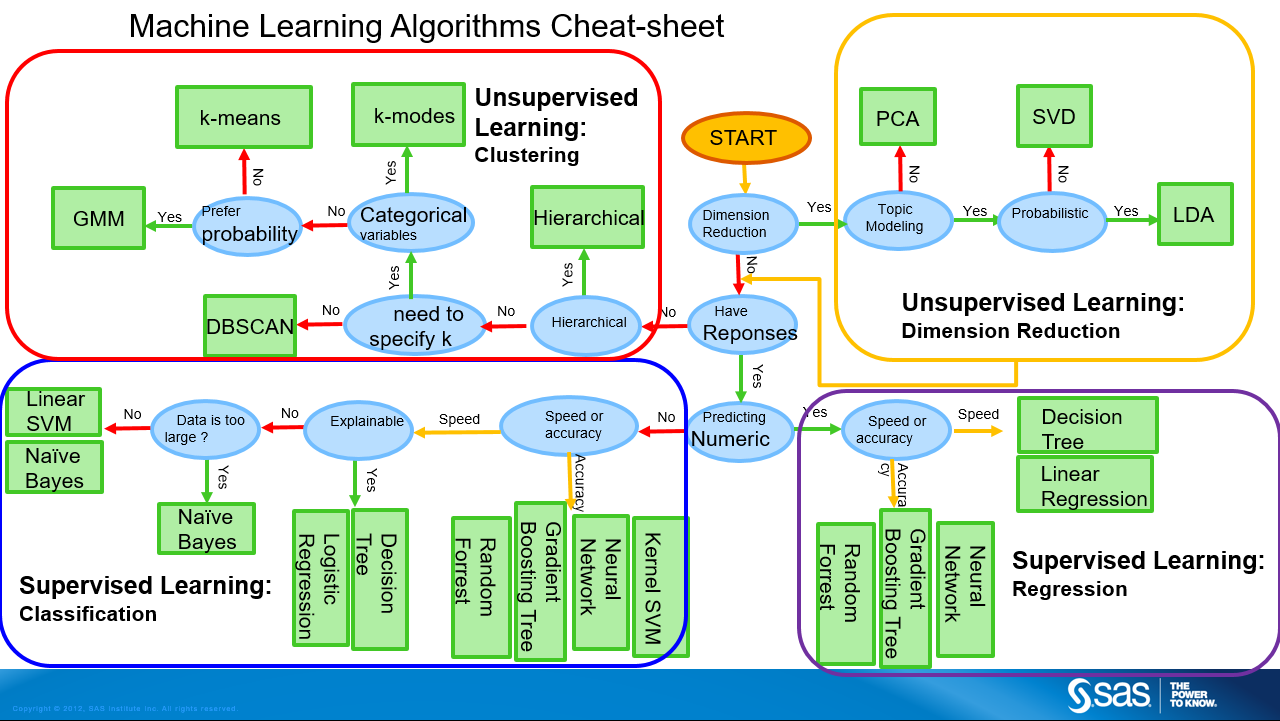
\includegraphics[width=0.12\linewidth]{../imgs/ml_algo} \end{center}

\hypertarget{machine-learning-algorithms-1}{%
\section{Machine Learning
Algorithms}\label{machine-learning-algorithms-1}}

\begin{itemize}
\tightlist
\item
  Regression
\item
  Classification
\item
  Ensemble
\item
  Neutral network

  \begin{itemize}
  \tightlist
  \item
    Deep learning
  \end{itemize}
\end{itemize}

\hypertarget{regression-and-classification}{%
\section{Regression and
Classification}\label{regression-and-classification}}

Regression and classification are two main categories of machine
learning algorithms.

\begin{center}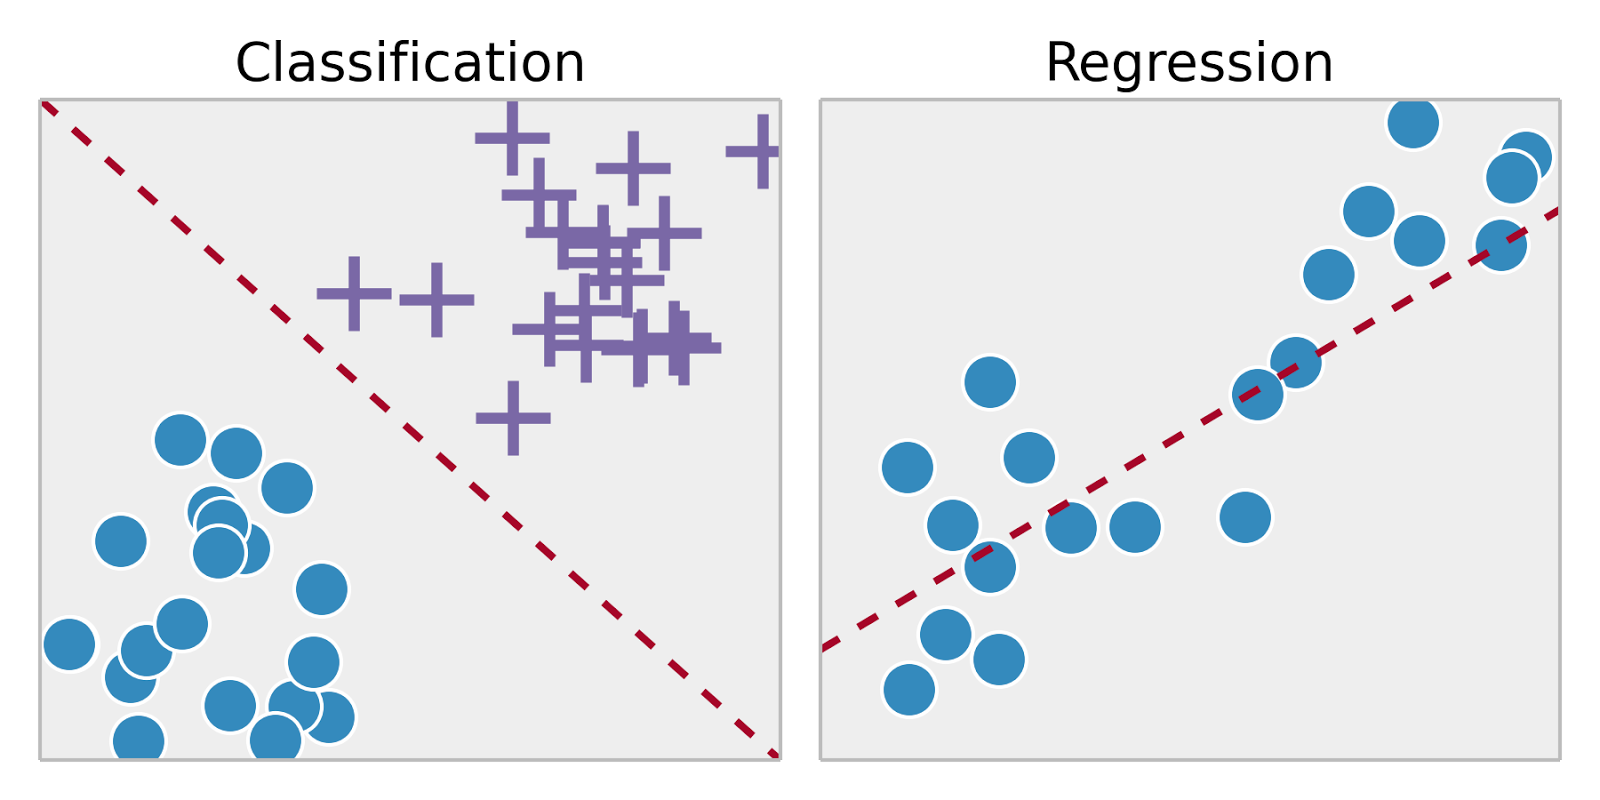
\includegraphics[width=0.12\linewidth]{../imgs/class_reg} \end{center}

One-hot encoding

Linear regression


\end{document}
